In the following part the quantities and tools used for contact analysis are briefly introduced.\\
\\
Intramolecular distances have been analysed with \conan{}. This analysis tool measures inter-residue distances and performs statistical analysis on them. \conan{} is still under development and not published yet.\\
The contact area of the FERM-kinase interface can be determined with the solvent accessible surface area (SASA) \autocite{sasaAlg} of the domains involved:
\begin{equation}
\text{CA} = \frac{1}{2} \left(\text{SASA}_\text{FERM} + \text{SASA}_\text{kinase} - \text{SASA}_\text{FERM-kinase}\right).
\end{equation}
For the calculation of SASA values \gromacs{} sasa tool was used. The v.d.W radii were adapted to \martini{} beads.\\
\\
For an appropriate description of intermolecular interactions between FAK molecules, we defined the following terms:\\
\textbf{Interaction} Proteins or part of proteins interact if their minimal distance is smaller than a cut-off distance (here $1.5\,\si{\nano\metre}$).\\
\textbf{Neighbour} Two proteins are neighbours if they are interacting with each other. One protein can have several neighbours. For a more detailed characterisation we defined the following neighbouring types (see \autoref{methods:inttypes}):
\begin{enumerate}[label={type \theenumi:}, leftmargin=*]
	\setcounter{enumi}{0}
	\item only the FERM domain interacts with only the FERM domain of the neighbouring protein
	\item only the kinase interacts with only the kinase of the neighbouring protein
	\item only the FERM domain interacts with only the kinase of the neighbouring protein
	\item the FERM domain is interacting with both, the FERM and kinase of the neighbouring protein
	\item the kinase is interacting with both, the FERM and kinase of the neighbouring protein
	\item the FERM domain is interacting with the FERM domain of the neighbouring protein and the kinase is interacting with the kinase of the neighbouring protein
	\item the FERM domain is interacting with the kinase of the neighbouring protein and the kinase is interacting with the FERM domain of the neighbouring protein
\end{enumerate}
It is important to see that the probability of the different types is initially biased, as the following example demonstrates. Assuming one FAK molecule with the FERM domain pointing to the right, a type 1 neighbour can only form if the second molecule docks via its FERM domain from the right. In contrast, a type 3 neighbour can still form from both sides with the appropriate orientations. Therefore, even if there would be no energetic preference between the interaction types, type 3 neighbours would be preferred. On the other hand, interactions of type 4, 5, 6 and 7 would occur more rarely, because the range of appropriate binding surfaces is much smaller compared to type 1, 2 and 3.
%
%
%
\begin{figure}
	\centering
	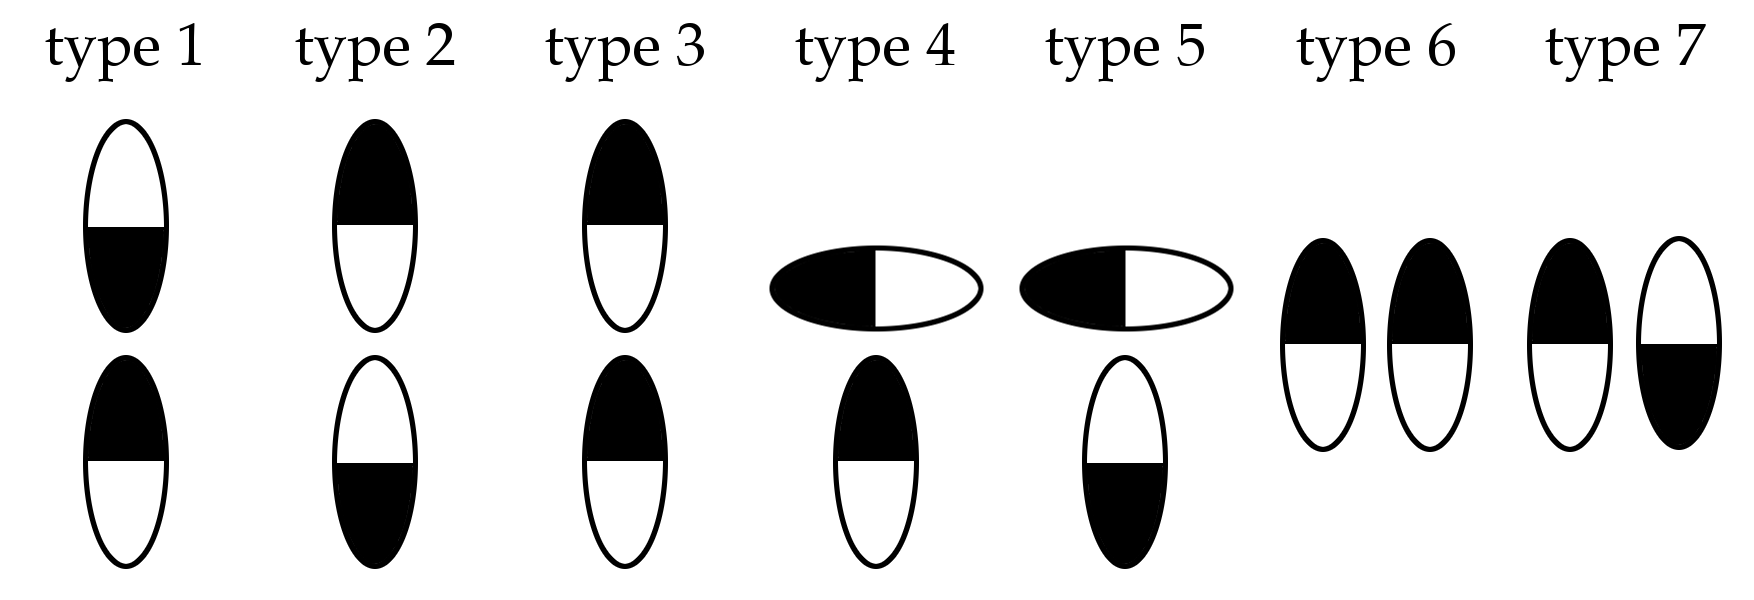
\includegraphics[width=0.6\textwidth]{figures/introduction/classification}
	\nicecaption{Neighbouring types}{The black part shows the FERM domain, the white the kinase. For type 4 and type 5, the upper protein can be vice versa as well.}
	\label{methods:inttypes}
\end{figure}
%
%
%